\section{Konversi Regular Expression ke NFA: Algoritma Thompson}

Algoritma Thompson adalah metode sistematis untuk mengkonversi regular expression menjadi $\epsilon$-NFA. Algoritma ini menggunakan pendekatan rekursif dengan template untuk setiap operasi regex.

\subsection{Template Dasar}

Algoritma Thompson menggunakan template untuk setiap operasi regex. Template-template berikut menunjukkan konstruksi dasar yang digunakan.

\subsubsection{Literal (Karakter Tunggal)}

Untuk regex \texttt{a}, NFA-nya adalah:

\begin{figure}[H]
    \centering
    \adjustbox{max width=0.5\textwidth,center}{%
    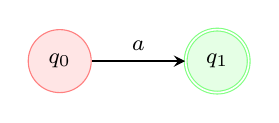
\begin{tikzpicture}[
        state/.style={circle, draw=blue!50, fill=blue!10, minimum size=0.8cm, font=\footnotesize},
        accept/.style={circle, draw=green!50, fill=green!10, minimum size=0.8cm, font=\footnotesize, double},
        start/.style={circle, draw=red!50, fill=red!10, minimum size=0.8cm, font=\footnotesize},
        arrow/.style={->, >=stealth, thick},
        node distance=2cm
    ]
    
    \node[start] (q0) at (0,0) {$q_0$};
    \node[accept] (q1) at (2,0) {$q_1$};
    \draw[arrow] (q0) -- node[above, font=\footnotesize] {$a$} (q1);
    
    \end{tikzpicture}%
    }
    \caption{Template NFA untuk literal \texttt{a}}
    \label{fig:thompson-literal}
\end{figure}

\subsubsection{Concatenation (RS)}

Untuk regex \texttt{RS}, NFA-nya dibangun dengan menghubungkan NFA untuk R dan S menggunakan $\epsilon$-transition:

\begin{figure}[H]
    \centering
    \adjustbox{max width=0.8\textwidth,center}{%
    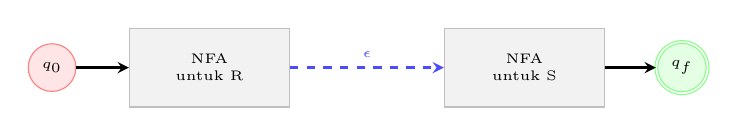
\begin{tikzpicture}[
        state/.style={circle, draw=blue!50, fill=blue!10, minimum size=0.6cm, font=\tiny},
        accept/.style={circle, draw=green!50, fill=green!10, minimum size=0.6cm, font=\tiny, double},
        start/.style={circle, draw=red!50, fill=red!10, minimum size=0.6cm, font=\tiny},
        box/.style={rectangle, draw=gray!50, fill=gray!10, text width=1.8cm, minimum height=1cm, font=\tiny, align=center},
        arrow/.style={->, >=stealth, thick},
        eps/.style={->, >=stealth, thick, dashed, blue!70},
        node distance=1.5cm
    ]
    
    \node[start] (q0) at (0,0) {$q_0$};
    \node[box] (nfaR) at (2,0) {NFA\\untuk R};
    \node (q1) at (4,0) {};
    \node[box] (nfaS) at (6,0) {NFA\\untuk S};
    \node[accept] (qf) at (8,0) {$q_f$};
    
    \draw[arrow] (q0) -- (nfaR);
    \draw[eps] (nfaR) -- node[above, font=\tiny] {$\epsilon$} (nfaS);
    \draw[arrow] (nfaS) -- (qf);
    
    \end{tikzpicture}%
    }
    \caption{Template NFA untuk concatenation \texttt{RS}}
    \label{fig:thompson-concat}
\end{figure}

\subsubsection{Union (R|S)}

Untuk regex \texttt{R|S}, NFA-nya menggunakan $\epsilon$-transitions untuk branching:

\begin{figure}[H]
    \centering
    \adjustbox{max width=0.7\textwidth,center}{%
    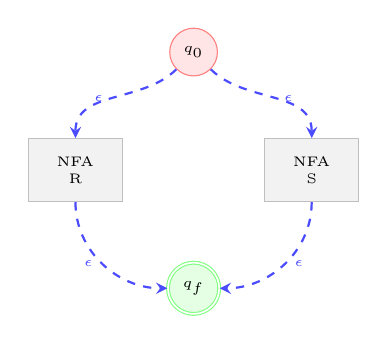
\begin{tikzpicture}[
        state/.style={circle, draw=blue!50, fill=blue!10, minimum size=0.6cm, font=\tiny},
        accept/.style={circle, draw=green!50, fill=green!10, minimum size=0.6cm, font=\tiny, double},
        start/.style={circle, draw=red!50, fill=red!10, minimum size=0.6cm, font=\tiny},
        box/.style={rectangle, draw=gray!50, fill=gray!10, minimum width=1.2cm, minimum height=0.8cm, font=\tiny, align=center},
        arrow/.style={->, >=stealth, thick},
        eps/.style={->, >=stealth, thick, dashed, blue!70},
        node distance=1.2cm
    ]
    
    \node[start] (q0) at (0,0) {$q_0$};
    \node[box] (nfaR) at (-1.5,-1.5) {NFA\\R};
    \node[box] (nfaS) at (1.5,-1.5) {NFA\\S};
    \node[accept] (qf) at (0,-3) {$q_f$};
    
    \draw[eps] (q0) to[out=225, in=90] node[left, font=\tiny] {$\epsilon$} (nfaR);
    \draw[eps] (q0) to[out=315, in=90] node[right, font=\tiny] {$\epsilon$} (nfaS);
    \draw[eps] (nfaR) to[out=270, in=180] node[left, font=\tiny] {$\epsilon$} (qf);
    \draw[eps] (nfaS) to[out=270, in=0] node[right, font=\tiny] {$\epsilon$} (qf);
    
    \end{tikzpicture}%
    }
    \caption{Template NFA untuk union \texttt{R|S}}
    \label{fig:thompson-union}
\end{figure}

\subsubsection{Kleene Star (R*)}

Untuk regex \texttt{R*}, NFA-nya memiliki loop dengan $\epsilon$-transitions:

\begin{figure}[H]
    \centering
    \adjustbox{max width=0.6\textwidth,center}{%
    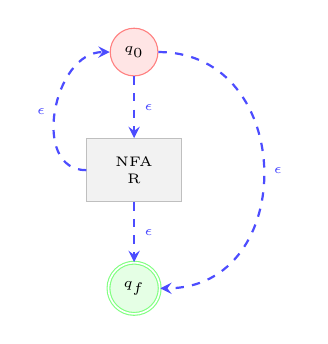
\begin{tikzpicture}[
        state/.style={circle, draw=blue!50, fill=blue!10, minimum size=0.6cm, font=\tiny},
        accept/.style={circle, draw=green!50, fill=green!10, minimum size=0.6cm, font=\tiny, double},
        start/.style={circle, draw=red!50, fill=red!10, minimum size=0.6cm, font=\tiny},
        box/.style={rectangle, draw=gray!50, fill=gray!10, minimum width=1.2cm, minimum height=0.8cm, font=\tiny, align=center},
        arrow/.style={->, >=stealth, thick},
        eps/.style={->, >=stealth, thick, dashed, blue!70},
        node distance=1.5cm
    ]
    
    \node[start] (q0) at (0,0) {$q_0$};
    \node[box] (nfaR) at (0,-1.5) {NFA\\R};
    \node[accept] (qf) at (0,-3) {$q_f$};
    
    % Epsilon transitions
    \draw[eps] (q0) -- node[right, font=\tiny] {$\epsilon$} (nfaR);
    \draw[eps] (nfaR) -- node[right, font=\tiny] {$\epsilon$} (qf);
    
    % Loop transitions
    \draw[eps] (q0) to[out=0, in=0, looseness=1.5] node[right, font=\tiny] {$\epsilon$} (qf);
    \draw[eps] (nfaR) to[out=180, in=180, looseness=1.2] node[left, font=\tiny] {$\epsilon$} (q0);
    
    \end{tikzpicture}%
    }
    \caption{Template NFA untuk Kleene star \texttt{R*}}
    \label{fig:thompson-kleene}
\end{figure}

\subsection{Contoh: Konversi \texttt{(a|b)*abb}}

Mari kita konstruksi NFA untuk regex \texttt{(a|b)*abb} menggunakan algoritma Thompson. Gambar \ref{fig:thompson-example} menunjukkan proses konstruksi langkah demi langkah.

\begin{enumerate}
    \item \textbf{Literal 'a' dan 'b'}: Buat NFA untuk masing-masing
    \item \textbf{Union (a|b)}: Gabungkan dengan $\epsilon$-transitions
    \item \textbf{Kleene Star ((a|b)*)}: Tambahkan loop dengan $\epsilon$-transitions
    \item \textbf{Concatenation dengan 'a'}: Tambahkan NFA untuk 'a'
    \item \textbf{Concatenation dengan 'b'}: Tambahkan NFA untuk 'b' (dua kali)
\end{enumerate}

\begin{figure}[H]
    \centering
    \adjustbox{max width=0.9\textwidth,center}{%
    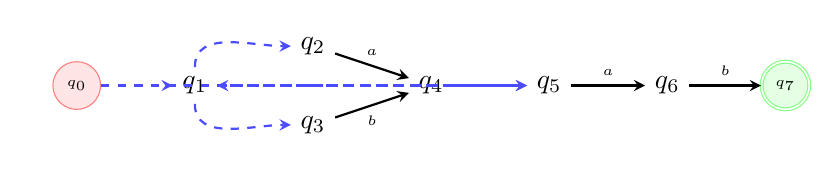
\begin{tikzpicture}[
        state/.style={circle, draw=blue!50, fill=blue!10, minimum size=0.5cm, font=\tiny},
        accept/.style={circle, draw=green!50, fill=green!10, minimum size=0.5cm, font=\tiny, double},
        start/.style={circle, draw=red!50, fill=red!10, minimum size=0.5cm, font=\tiny},
        arrow/.style={->, >=stealth, thick},
        eps/.style={->, >=stealth, thick, dashed, blue!70},
        node distance=0.8cm
    ]
    
    % Start
    \node[start] (q0) at (0,0) {$q_0$};
    
    % (a|b)* part
    \node (q1) at (1.5,0) {$q_1$};
    \node (q2) at (3,0.5) {$q_2$};
    \node (q3) at (3,-0.5) {$q_3$};
    \node (q4) at (4.5,0) {$q_4$};
    
    % 'a' part
    \node (q5) at (6,0) {$q_5$};
    
    % 'b' parts
    \node (q6) at (7.5,0) {$q_6$};
    \node[accept] (q7) at (9,0) {$q_7$};
    
    % Transitions for (a|b)*
    \draw[eps] (q0) -- (q1);
    \draw[eps] (q1) to[out=90, in=180] (q2);
    \draw[eps] (q1) to[out=270, in=180] (q3);
    \draw[arrow] (q2) -- node[above, font=\tiny] {$a$} (q4);
    \draw[arrow] (q3) -- node[below, font=\tiny] {$b$} (q4);
    \draw[eps] (q4) to[out=0, in=0, looseness=2] (q1);
    \draw[eps] (q4) -- (q5);
    
    % 'a' transition
    \draw[arrow] (q5) -- node[above, font=\tiny] {$a$} (q6);
    
    % 'b' transitions
    \draw[arrow] (q6) -- node[above, font=\tiny] {$b$} (q7);
    
    % Direct path from start to accept (for empty string)
    \draw[eps] (q0) to[out=0, in=180, looseness=3] (q5);
    
    \end{tikzpicture}%
    }
    \caption{NFA untuk regex \texttt{(a|b)*abb} menggunakan algoritma Thompson}
    \label{fig:thompson-example}
\end{figure}

Hasil akhirnya adalah NFA yang dapat mengenali string seperti ``abb'', ``aabb'', ``babb'', ``ababb'', dll. NFA ini memiliki $\epsilon$-transitions yang memungkinkan multiple paths untuk input yang sama.